\documentclass[11pt]{article}
\setlength{\topmargin}{-1.5cm}
\setlength{\textheight}{23cm}
\setlength{\oddsidemargin}{0mm}
\setlength{\evensidemargin}{0mm}
\setlength{\textwidth}{17cm}
\usepackage{graphicx, color}
\usepackage{amsmath, amssymb, amsthm}
\usepackage{verbatim}
\usepackage{tipa}

\begin{document}
\noindent {\large  \textbf{Shawn Pan - CS 222 Homework 2}}

\medskip

\noindent \textbf{Code is attached at the end of this document.}

\medskip

\noindent \textbf{Problem 1}

We compared gzip (DEFLATE = LZ77 + Huffman), bzip2 (Burrows-Wheeler), xz (LZMA2), and 7zip with the PPM option.

The files we compared included 10MB of random bits, 10MB of 0 bits, text of Alice in Wonderland, a $200 \times 101$ table of numerical data, minimized Javascript code, a PNG image, an mp3 music file, an mp4 video, and parts of a dump of Wikipedia ranging from 1KB to 1GB.  The inspiration to use Wikipedia came from this site which has a collection of text compression benchmarks (http://mattmahoney.net/dc/text.html).

Our results show that all the utilities sucessfully compressed text based data by a factor of 3 to 5.  However, the media files essentially did not compress at all.  As expected, random bits cannot be compressed, and identical zero bits can be compressed almost perfectly.  gzip, bzip2, and xz took longer to compress than decompress in general, while ppm was symmetric.  Prediction by partial matching (7zip) achieved the best text compression rates.  LZ77 (gzip) achieved the fastest times.  All the algorithms run in approximately linear time as shown by trend in Wikipedia dumps.  Also, larger text files achieved better compression ratios, presumably because more patterns could be exploited.

\begin{table}[h!]
\caption{Compressed Sizes (bytes) and Compression Ratios}
\small
\begin{tabular}{| l | r | r r | r r | r r | r r |}
\hline
File & Original & gzip & ratio & bzip2 & ratio & xz & ratio & 7z ppmd & ratio\\
\hline
random & 10000000 & 10001555 & 1.0002 & 10044419 & 1.0044 & 10000560 & 1.0001 & 10228516 & 1.0229\\
zero & 10000000 & 9742 & 0.0010 & 49 & 0.0000 & 1584 & 0.0002 & 3791 & 0.0004\\
\hline
alice.txt & 173595 & 61370 & 0.3535 & 49144 & 0.2831 & 54072 & 0.3115 & 44065 & 0.2538\\
numeric.csv & 505009 & 217219 & 0.4301 & 182355 & 0.3611 & 188288 & 0.3728 & 183292 & 0.3629\\
jquery.js & 86709 & 29979 & 0.3457 & 27530 & 0.3175 & 28292 & 0.3263 & 24932 & 0.2875\\
image.png & 736501 & 736514 & 1.0000 & 739754 & 1.0044 & 736600 & 1.0001 & 752219 & 1.0213\\
music.mp3 & 4426883 & 4385198 & 0.9906 & 4370711 & 0.9873 & 4365156 & 0.9861 & 4386499 & 0.9909\\
video.mp4 & 905296268 & 904838573 & 0.9995 & 908527162 & 1.0036 & 904758648 & 0.9994 & 925040248 & 1.0218\\
\hline
enwik3 & 1000 & 343 & 0.3430 & 391 & 0.3910 & 400 & 0.4000 & 408 & 0.4080\\
enwik4 & 10000 & 3728 & 0.3728 & 3733 & 0.3733 & 3656 & 0.3656 & 3393 & 0.3393\\
enwik5 & 100000 & 36145 & 0.3615 & 31372 & 0.3137 & 33000 & 0.3300 & 28115 & 0.2812\\
enwik6 & 1000000 & 356264 & 0.3563 & 281323 & 0.2813 & 290692 & 0.2907 & 250071 & 0.2501\\
enwik7 & 10000000 & 3693807 & 0.3694 & 2916026 & 0.2916 & 2723036 & 0.2723 & 2491710 & 0.2492\\
enwik8 & 100000000 & 36518329 & 0.3652 & 29008758 & 0.2901 & 26375764 & 0.2638 & 24849802 & 0.2485\\
enwik9 & 1000000000 & 323742882 & 0.3237 & 253977891 & 0.2540 & 230153052 & 0.2302 & 219169705 & 0.2192\\
\hline
\end{tabular}
\end{table}

\begin{table}[h!]
\caption{Compression and Decompression Times (CPU seconds)}
\small
\begin{tabular}{| l | r r | r r | r r | r r |}
\hline
 & gzip &  & bzip2 &  & xz &  & 7z ppmd & \\
File & compress & decompress & compress & decompress & compress & decompress & compress & decompress\\
\hline
random & 0.32 & 0.076 & 1.368 & 0.624 & 2.848 & 0.04 & 3.832 & 4.772\\
zero & 0.064 & 0.064 & 0.092 & 0.052 & 0.508 & 0.052 & 0.132 & 0.172\\
\hline
alice.txt & 0.008 & 0 & 0.012 & 0.004 & 0.052 & 0.004 & 0.02 & 0.02\\
numeric.csv & 0.036 & 0.004 & 0.04 & 0.02 & 0.172 & 0.02 & 0.064 & 0.072\\
jquery.js & 0.004 & 0 & 0.008 & 0.004 & 0.024 & 0 & 0.012 & 0.012\\
image.png & 0.024 & 0.004 & 0.1 & 0.044 & 0.148 & 0.004 & 0.264 & 0.336\\
music.mp3 & 0.164 & 0.044 & 0.58 & 0.268 & 1.104 & 0.296 & 1.688 & 2.088\\
video.mp4 & 28.76 & 6.628 & 122.92 & 60.684 & 295.46 & 4.02 & 341.268 & 432.116\\
\hline
enwik3 & 0 & 0 & 0 & 0 & 0 & 0 & 0 & 0\\
enwik4 & 0 & 0 & 0 & 0 & 0.004 & 0 & 0 & 0.004\\
enwik5 & 0.004 & 0 & 0.008 & 0.004 & 0.028 & 0 & 0.012 & 0.012\\
enwik6 & 0.044 & 0.008 & 0.084 & 0.036 & 0.328 & 0.02 & 0.096 & 0.116\\
enwik7 & 0.456 & 0.092 & 0.824 & 0.36 & 5.156 & 0.184 & 1.024 & 1.18\\
enwik8 & 4.64 & 0.892 & 8.296 & 3.704 & 60.464 & 1.796 & 10.5 & 11.988\\
enwik9 & 41.464 & 8.78 & 85.788 & 35.452 & 537.176 & 16.376 & 96.168 & 106.332\\
\hline
\end{tabular}
\end{table}

\pagebreak

\noindent \textbf{Problem 2}

For $X=n$, the coin must land on tails $n-1$ times follwed by heads.
Each coin flip happens independently with probability $\frac12$, so the probability $X=n$ is $2^{-n}$.

\begin{align*}
H &= -\sum_{n=1}^\infty 2^{-n} \log_2 2^{-n}\\
&= \sum_{n=1}^\infty n 2^{-n}\\
&= (1)\frac12 + (2)\frac14 + (3)\frac18 + \dots\\
2H &= (1)1 + (2)\frac12 + (3)\frac14 + (4)\frac18 + \dots\\
2H - H &= (1-0)1 + (2-1)\frac12 + (3-2)\frac14 + (4-3)\frac18 + \dots\\
H &= 1 + \frac12 + \frac14 + \frac18 + \dots\\
&= \frac{1}{1 - \frac12}\\
&= 2
\end{align*}

The optimal series of questions to ask are ``Is X = 1?'' ``Is X = 2?'' ``Is X = 3?'' ...
With probablity $\frac12$ you are correct on your first question.  Otherwise, with probability $(\frac12)(\frac12)$ you will be correct on your second questions, and so on.
The expected number of questions asked is $E = \sum_{n=1}^\infty n 2^{-n} = 2$, which is the same infinite series as the entropy calculation above.  As expected $H = E$.

\pagebreak

\noindent \textbf{Problem 3}

\medskip

\noindent \textbf{Show $H(Z|X) = H(Y|X)$}

\begin{align*}
H(Z|X) &= \sum_x P(X=x) \sum_z P(Z=z|X=x) \log_2 P(Z=z|X=x)\\
&= \sum_x P(X=x) \sum_z P(X+Y=z|X=x) \log_2 P(X+Y=z|X=x)\\
&= \sum_x P(X=x) \sum_{y=z-x} P(Y=z-x|X=x) \log_2 P(Y=z-x|X=x)\\
&= \sum_x P(X=x) \sum_y P(Y=y|X=x) \log_2 P(Y=y|X=x)\\
&= H(Y|X)
\end{align*}

\medskip

\noindent \textbf{Show $H(Z) \ge H(X)$ when X and Y are independent}

The marginal entropy $H(Z)$ must be at least the conditional entropy $H(Z | Y)$.  By symmetry of the case above, $H(Z | Y) = H(X | Y)$.  Because of independence, $H(X | Y) = H(X)$.
$$H(Z) \ge H(Z | Y) = H(X | Y) = H(X)$$

\medskip

\noindent \textbf{Example $H(X) > H(Z)$}

Consider the case $X = 1, 2, 3, ..., r$ with equal probabilities $\frac1r$ and $Y = -X$.  $Z = X + Y = 0$ everywhere, so $H(Z) = 0$.  However, $H(X) = \log_2 r > 0 = H(Z)$.

\medskip

\noindent \textbf{Conditions for $H(Z) = H(X) + H(Y)$}

$H(Z) = H(X) + H(Y)$ when $X$ and $Y$ are independent and all sums $z_{ij} = x_i + y_j$ are distinct.  Intuitively, for $Z$ to have the same information content as $X$ and $Y$ independently combined, we must be able to recover x and y given a z.

We will show that these 2 conditions are sufficient.  The key is that $P(z_{ij}) = P(x_i)P(y_j)$ because of independence and distinctness.
\begin{align*}
H(Z) &= - \sum_z P(z) \log_2 P(z)\\
&= - \sum_x \sum_y P(x)P(y) \log_2 P(x)P(y)\\
&= - \sum_x \sum_y P(x)P(y) \left( \log_2 P(x) +  \log_2 P(y) \right)\\
&= - \sum_x \sum_y P(x)P(y) \log_2 P(x) - \sum_x \sum_y P(x)P(y) \log_2 P(y)\\
&= - \sum_y P(y) \sum_x P(x) \log_2 P(x) - \sum_x P(x) \sum_y P(y) \log_2 P(y)\\
&= - \sum_x P(x) \log_2 P(x) - \sum_y P(y) \log_2 P(y)\\
&= H(X) + H(Y)
\end{align*}

\pagebreak

Note that both these conditions are necessary as shown by these two counterexamples:
\begin{enumerate}
\item Consider independent $X = {0, 1}$ and $Y = {0, 1}$ with equal probability for each option.  Note that two of the pairs sum to 1, and $Z = {0, 1, 2}$ with probabilties ${0.25, 0.5, 0.25}$.  $H(X) = H(Y) = 1$ and $H(Z) = 1.5 \ne H(X) + H(Y)$.
\item Consider $X = {1, 2}$ with equal probability and $Y = 2X = {2, 4}$.  $Z = {3, 4, 5, 6}$ with probabilities ${0.5, 0, 0, 0.5}$.  $H(X) = H(Y) = H(Z) = 1$ and $H(Z) \ne H(X) + H(Y)$.
\end{enumerate}

\medskip

\noindent \textbf{Problem 4}

Consider any pair of 2 faces of the die.  Let $p + \epsilon$ and $p - \epsilon$ be the probabilites of landing on the those 2 faces.  Note that the sum is a constant $2p$ independent of $\epsilon$, and we want to figure out how to distribute the probability by varying $\epsilon$ to maximize entropy.

\begin{align*}
H &= - (p + \epsilon) \log_2 (p + \epsilon) - (p - \epsilon) \log_2 (p - \epsilon)\\
\frac{dH}{d\epsilon} &= - \log_2 (p + \epsilon) - (p + \epsilon) \frac{1}{\ln 2} \frac{1}{p + \epsilon} + \log_2 (p - \epsilon) + (p - \epsilon) \frac{1}{\ln 2} \frac{1}{p - \epsilon}\\
&= \log_2 \left( \frac{p - \epsilon}{p + \epsilon} \right)\\
&= 0\\
\frac{p - \epsilon}{p + \epsilon} &= 1\\
\epsilon &= 0\\
\frac{d^2H}{d\epsilon^2} &= \left( \frac{1}{\ln 2} \right) \left( \frac{p + \epsilon}{p - \epsilon} \right) \left( \frac{-(p + \epsilon)-(p - \epsilon)}{(p + \epsilon)^2} \right)\\
&= \frac{-2p}{\ln 2(p + \epsilon)(p - \epsilon)}\\
&< 0
\end{align*}

The derivative is 0 when $\epsilon = 0$, and that point is a maximum because the second derivative is negative.  Therefore, entropy is maximized by splitting probabilities equally between 2 faces.  By considering all pairs of faces, we can generalize the result to say the entropy of a die is maximized when all faces have equal probability.

\pagebreak

\noindent \textbf{Problem 5}

First we append an end-of-file character to the input and generate all the cyclic shifts.

\begin{verbatim}
wabbawabbawoo|
abbawabbawoo|w
bbawabbawoo|wa
bawabbawoo|wab
awabbawoo|wabb
wabbawoo|wabba
abbawoo|wabbaw
bbawoo|wabbawa
bawoo|wabbawab
awoo|wabbawabb
woo|wabbawabba
oo|wabbawabbaw
o|wabbawabbawo
|wabbawabbawoo
\end{verbatim}

Then we sort the shifts alphabetically.

\begin{verbatim}
abbawabbawoo|w
abbawoo|wabbaw
awabbawoo|wabb
awoo|wabbawabb
bawabbawoo|wab
bawoo|wabbawab
bbawabbawoo|wa
bbawoo|wabbawa
oo|wabbawabbaw
o|wabbawabbawo
wabbawabbawoo|
wabbawoo|wabba
woo|wabbawabba
|wabbawabbawoo
\end{verbatim}

We output the last column wwbbbbaawo\textpipe aao.

So far, we have simply transformed the data.  The first column has been sorted and is a good predictor for the last column which is cyclicly adjacent.  Therefore, the last column should have clusters of characters and can be compressed by move-to-front encoding.  We start with a dictionary of all the characters and move them to the front each time a character is used.

\begin{verbatim}
['a', 'b', 'o', 'w', '|'] [3]
['w', 'a', 'b', 'o', '|'] [3, 0]
['w', 'a', 'b', 'o', '|'] [3, 0, 2]
['b', 'w', 'a', 'o', '|'] [3, 0, 2, 0]
['b', 'w', 'a', 'o', '|'] [3, 0, 2, 0, 0]
['b', 'w', 'a', 'o', '|'] [3, 0, 2, 0, 0, 0]
['b', 'w', 'a', 'o', '|'] [3, 0, 2, 0, 0, 0, 2]
['a', 'b', 'w', 'o', '|'] [3, 0, 2, 0, 0, 0, 2, 0]
['a', 'b', 'w', 'o', '|'] [3, 0, 2, 0, 0, 0, 2, 0, 2]
['w', 'a', 'b', 'o', '|'] [3, 0, 2, 0, 0, 0, 2, 0, 2, 3]
['o', 'w', 'a', 'b', '|'] [3, 0, 2, 0, 0, 0, 2, 0, 2, 3, 4]
['|', 'o', 'w', 'a', 'b'] [3, 0, 2, 0, 0, 0, 2, 0, 2, 3, 4, 3]
['a', '|', 'o', 'w', 'b'] [3, 0, 2, 0, 0, 0, 2, 0, 2, 3, 4, 3, 0]
['a', '|', 'o', 'w', 'b'] [3, 0, 2, 0, 0, 0, 2, 0, 2, 3, 4, 3, 0, 2]
\end{verbatim}

The output of the move-to-front encoding [3, 0, 2, 0, 0, 0, 2, 0, 2, 3, 4, 3, 0, 2] can be efficiently encoded with Huffman or arithmetic coding.

\medskip

To decoder receives the encoded last column.  The move-to-front procedure is applied in reverse to recover the last column wwbbbbaawo\textpipe aao.  We determine the index of correct row (10) by finding the end-of-file character \textpipe~in the last column.  We sort the last column to recover the first column aaaabbbboowww\textpipe.  Note that the last and first columns together form all the pairs in the original data.

\begin{align*}
w_1a_1\\
w_2a_2\\
b_1a_3\\
b_2a_4\\
b_3b_1\\
b_4b_2\\
a_1b_3\\
a_2b_4\\
w_3o_1\\
o_1o_2\\
|_1w_1\\
a_3w_2\\
a_4w_3\\
o_2|_1
\end{align*}

If we index the identical characters in order, we can follow these pairs along a chain to recover any row.
$$|_1w_1 \rightarrow w_1a_1 \rightarrow a_1b_3 \rightarrow b_3b_1 \rightarrow b_1a_3 \rightarrow a_3w_2 \rightarrow w_2a_2 \rightarrow a_2b_4 \rightarrow b_4b_2 \rightarrow b_2a_4 \rightarrow a_4w_3 \rightarrow w_3o_1 \rightarrow o_1o_2$$

We recover the original phrase wabbawabbawoo.

\pagebreak

\noindent \textbf{Problem 6}

\begin{verbatim}
Encode
(0.0, 0.2, 1)
(0.0, 0.04000000000000001, 2)
(0.020000000000000004, 0.04000000000000001, 3)
(0.024000000000000004, 0.030000000000000006, 4)
(0.027000000000000003, 0.030000000000000006, 5)
(0.027000000000000003, 0.027600000000000003, 6)
\end{verbatim}

The interval from $[0.027, 0.0276)$. To prevent rounding errors, it's probably safest to output the midpoint of the interval.  If rounding were not a concern 0.027 would be shorter.
We transmit \textbf{0.0273} and the length \textbf{6}.

\begin{verbatim}
Decode
c 0.26431398
cb 0.214379933333
cbb 0.0479331111111
cbba 0.239665555556
cbbab 0.132218518519
cbbaba 0.661092592593
cbbabac 0.322185185185
cbbabacb 0.407283950618
cbbabacbb 0.690946502059
cbbabacbbc 0.381893004117
\end{verbatim}

To decode we rescale the interval at each step and end up with \textbf{cbbabacbbc}.

\medskip

\noindent \textbf{Problem 7}

\noindent \textbf{Forward Result}

S: BCBaCHtHg, B: aE, C: tg, D: ag, E: ac, H: DDEa

\noindent \textbf{Backward Result}

S: ADEDgEGgtG, A: ga, D: FAA, E: ta, F: ca, G: Fa

\noindent \textbf{Step-by-step output of my code}
\verbatiminput{hw2_7.out}

\medskip

\noindent \textbf{Problem 8}
\verbatiminput{hw2_8.out}

\begin{figure}[h!]
  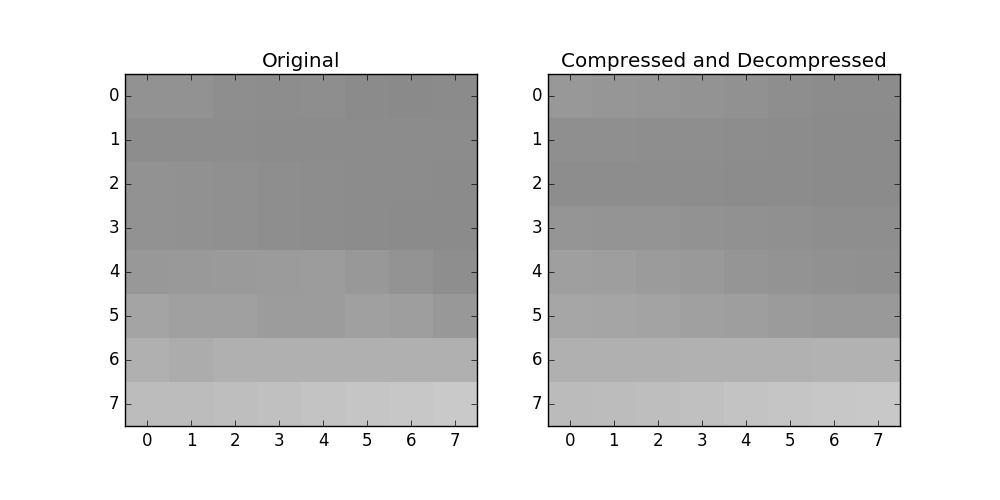
\includegraphics[width=7in]{jpegtest.png}
\end{figure}

JPEG appears to compress well by reducing most components to zero, but visibly blurs the sharp edges in the original block.

\pagebreak

\noindent \textbf{Problem 9}

\verbatiminput{hw2_9.out}

For LZ77, if multiple matches of the same length occur in the window, I'm taking the smallest offset (rightmost) match, which I believe is the match that the original paper used and could potentially be compressed more.  The example on Wikipedia appears to take the opposite convention of taking the first (leftmost) match.  Following that convention, you would get the following output.

\begin{verbatim}
(0, 0, 'a')
(0, 0, 'b')
(0, 0, 'r')
(3, 1, 'c')
(5, 1, 'd')
(4, 1, 'b')
(0, 0, 'r')
(5, 1, 'a')
(3, 1, 'b')
(4, 1, 'd')
(6, 1, 'c')
(4, 1, 'r')
(0, 0, 'b')
(5, 1, None)
\end{verbatim}

\pagebreak

\noindent \textbf{Problem 10}

We have enough information to reconstruct the numbers because we can find each number by adding the difference to the previous number $a_i = a_{i-1} + d_{i-1,i}$ and we have $a_0$ as the base case to start the chain.

\begin{verbatim}
bits used: 210014 k: 21
bits used: 200015 k: 20
bits used: 210014 k: 21
bits used: 200015 k: 20
bits used: 200015 k: 20
bits used: 210014 k: 21
bits used: 210014 k: 21
bits used: 210014 k: 21
bits used: 210014 k: 21
bits used: 210014 k: 21
\end{verbatim}

Consider $m=1$.  The left half contains only 0 and 1, and is very easy to compress.  We could just transmit the count of zeros and ones to recover the left half, because the entries are sorted.  However, this scheme is very inefficient for the right half, since we would need 29 bits each.

We will extend the idea of transmitting counts of each possible left half.  The optimal number of bins appears to be around $m=13$ where the number of bins $2^{13}=8192$ is approximately the data size $10000$.  Because the numbers are random, with high probability they contain a small number of entries and require only $\lceil\log_2 c\rceil$ bits each where $c$ is the maximum count of a bin.  This is enough information to recover the left half because we have the run length of every possible left half in sequence.  We can combine the left and right halves to recover all original numbers.  For the case of random inputs, transmitting all $2^{13}$ counts turns out to be more efficient than transmitting pairs of (value, run length) because most of the $2^{13}$ possible values have non-zero counts.

The total number of bits required is $n(30 - m) + 2^m\lceil\log_2 c\rceil)$, plus or minus a few bits, depending on the exact implementation.  You could transmit the bits per bin or some end-of-file symbol to recover the bits per bin.  You could also get away with not transmitting one of the counts if you know the total data size.

\begin{verbatim}
bits used: 194590 bits per bin: 3
bits used: 194590 bits per bin: 3
bits used: 202782 bits per bin: 4
bits used: 194590 bits per bin: 3
bits used: 194590 bits per bin: 3
bits used: 194590 bits per bin: 3
bits used: 194590 bits per bin: 3
bits used: 194590 bits per bin: 3
bits used: 194590 bits per bin: 3
bits used: 194590 bits per bin: 3
\end{verbatim}

\pagebreak

\noindent \textbf{Problem 1 Code}
\verbatiminput{hw2_1.py}

\pagebreak

\noindent \textbf{Problem 5 Code}
\verbatiminput{hw2_5.py}

\pagebreak

\noindent \textbf{Problem 6 Code}
\verbatiminput{hw2_6.py}

\pagebreak

\noindent \textbf{Problem 7 Code}
\verbatiminput{hw2_7.py}

\pagebreak

\noindent \textbf{Problem 8 Code}
\verbatiminput{hw2_8.py}

\pagebreak

\noindent \textbf{Problem 9 Code}
\verbatiminput{hw2_9.py}

\pagebreak

\noindent \textbf{Problem 10 Code}
\verbatiminput{hw2_10.py}

\end{document}